\section{Elements of CNN}

\subsection{Understanding the convolutional layer}
\textbf{Problem : Implement the convolutional layer method by hand} \\

\begin{figure}[ht]
  \centering
  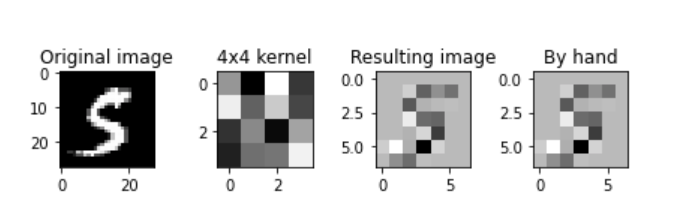
\includegraphics{Pics/convolutionn}
  \caption{Convolution plot}
\end{figure}
In this case we apply a $4 \times 4$ (K) kernel on the $28 \times 28$ (N) input picture (greyscale). The stride, or step size is $(4,4)$ (S). It means that we go through the input picture with a $4\times 4$ rolling windows that computes the weighted sum of the pixel values. The resulting feature map is a $\frac{N-K}{S}=\frac{28-4}{4}+1=7$ by 7 output picture. We do this hand convolution as follows : 
\begin{lstlisting}[language=Python]
np_image = image[0][0].data.numpy()
image_conv = np.zeros((7,7))
for i in range(7):
    for j in range(7):
        image_conv[i, j]=np.sum(np_image[(4*i):(4*i+4), (4*j):(4*j+4)] * weight)

\end{lstlisting}


\section{Problem 2 : Dropout}

\textbf{Question: Modify the code for ConvNet and insert Dropout layer (wherever you want)}.\\
	The dropout allows us to shut down parts of the neural networks to prevent from over-fitting. A fully connected layer occupies most of the parameters so it risks to favour co-dependency between neurons during the train phase. This would result in poor performances on held-out test data.\\
It's a regularization approach which allows us to reduce interdependency (also called co-adaptation) between neurons with a view to increasing robustness of the model. This approach looks alike the Random Forest with iterated random features and data selections. But here, we will be randomly deactivating p*node on each layer and at each iteration.  \\

More precisely :
\begin{itemize}
\item During the training phase, for each hidden layer, for each training sample, for each iteration, we will ignore nodes (by "zeroing" them) with a probability p using samples from a Bernoulli distribution.

\item During the testing phase, we will use (1-p) activations to take into account the missing nodes (hence activations) during the training phase.
\end{itemize}

The method dropout in Pytorch takes two arguments, the first one is p the probability of node dropout which is set by default to 0.5 (following the paper by Hinton et Al. in 2012). The second one is inplace set by default to False. We decide to use the \verb|Dropout2d| function that works on the level of the channels. It will randomly set to zero entire channels (entire feature maps).  We put it just after the convolutional layer. Indeed, the convolution layer has extended the channel size of the output from 1 to 8. \\
\begin{figure}[ht]
  \centering
  \includegraphics[scale=0.3]{Pics/dropout}
  \caption{Neural Network plot}
\end{figure}

As the figure 2 suggests, we use a convolutionnal layer, followed by the dropout, a ReLu activation and a Max-Pool to diminish the dimension of the data. Then the output is flattened in a $1\times 500$ vector and passed through a ReLu activation before the last linear transformation that takes the $1\times 500$ vector and diminishes it into a $1\times 10$ vector for the 10 different possible outputs. 
